\documentclass[11pt,a4paper]{article}
\usepackage{amsmath}
\usepackage{amssymb}
\usepackage{geometry}
\usepackage{hyperref}
\usepackage{listings}
\usepackage{xcolor}
\usepackage{graphicx}
\usepackage{float}
\usepackage{tikz}
\usetikzlibrary{shapes,arrows,positioning,calc,shapes.geometric,shapes.multipart}

\geometry{margin=0.8in}

\lstset{
  language=Python,
  basicstyle=\ttfamily\small,
  breaklines=true,
  commentstyle=\color{gray},
  keywordstyle=\color{blue},
  stringstyle=\color{red},
  tabsize=2,
  frame=single,
  backgroundcolor=\color{white!95!black}
}

\title{Architecture Guide: Physics-Informed Transformer\\Schematic \& Code Details}
\author{}
\date{}

\begin{document}

\maketitle
\tableofcontents
\newpage

\section{Quick Reference: Dimensions}

\begin{table}[H]
\centering
\begin{tabular}{|c|c|l|}
\hline
\textbf{Symbol} & \textbf{Value} & \textbf{Meaning} \\
\hline
$B$ & 16 & Batch size (samples per training iteration) \\
$T$ & 50 & Time steps (load history length) \\
$D$ & 64 & Embedding dimension (internal representation) \\
$N$ & 8 & Soil parameters (input features) \\
$n$ & 20 & Yield surfaces (degradation stages) \\
\hline
\end{tabular}
\end{table}

\section{Architecture Overview}

\subsection{Top-Level Flow}

\begin{figure}[H]
\centering
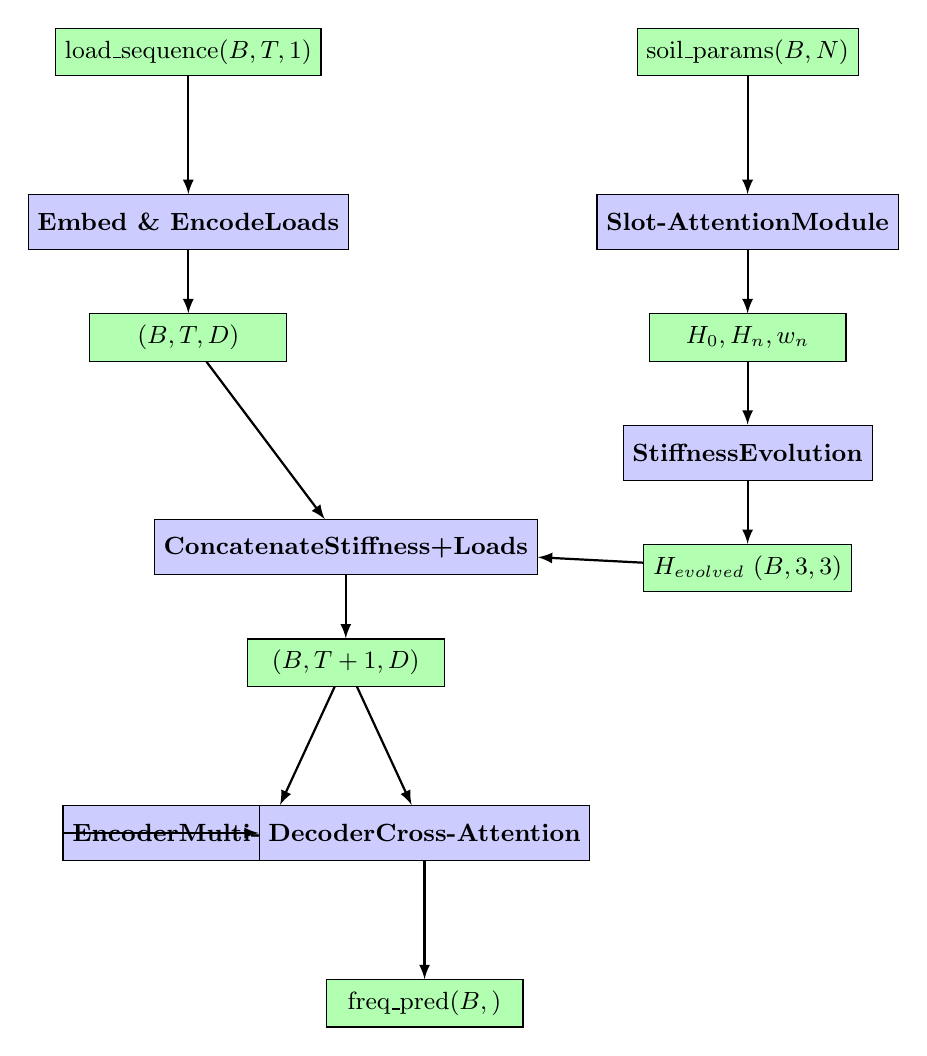
\begin{tikzpicture}[
  node distance=1.5cm,
  box/.style={rectangle, draw, fill=blue!20, minimum width=2.5cm, minimum height=0.7cm, font=\small\bfseries},
  input/.style={rectangle, draw, fill=green!30, minimum width=2.5cm, minimum height=0.6cm, font=\small},
  arrow/.style={->, >=latex, thick}
]

% Input
\node[input] (inp1) {load\_sequence\\$(B,T,1)$};
\node[input] (inp2) [right=4cm of inp1] {soil\_params\\$(B,N)$};

% Branch 1: Load side
\node[box] (emb) [below=1.5cm of inp1] {Embed \& Encode\\Loads};
\draw[arrow] (inp1) -- (emb);

\node[input] (emb_out) [below=0.8cm of emb] {$(B,T,D)$};
\draw[arrow] (emb) -- (emb_out);

% Branch 2: Soil side
\node[box] (slot) [below=1.5cm of inp2] {Slot-Attention\\Module};
\draw[arrow] (inp2) -- (slot);

\node[input] (stiff_out) [below=0.8cm of slot] {$H_0, H_n, w_n$};
\draw[arrow] (slot) -- (stiff_out);

\node[box] (evol) [below=0.8cm of stiff_out] {Stiffness\\Evolution};
\draw[arrow] (stiff_out) -- (evol);

\node[input] (h_evo) [below=0.8cm of evol] {$H_{evolved}$ $(B,3,3)$};
\draw[arrow] (evol) -- (h_evo);

% Merge
\node[box] (concat) [below=2cm of emb_out, xshift=2cm] {Concatenate\\Stiffness+Loads};
\draw[arrow] (emb_out) -- (concat);
\draw[arrow] (h_evo) -- (concat);

\node[input] (merged) [below=0.8cm of concat] {$(B,T+1,D)$};
\draw[arrow] (concat) -- (merged);

% Transformer
\node[box] (encoder) [below=1.5cm of merged, xshift=-1cm] {Encoder\\Multi-Head Attention};
\draw[arrow] (merged) -- (encoder);

\node[box] (decoder) [below=1.5cm of merged, xshift=1cm] {Decoder\\Cross-Attention};
\draw[arrow] (merged) -- (decoder);
\draw[arrow] (encoder) -- (decoder);

% Output
\node[input] (output) [below=1.5cm of decoder] {freq\_pred\\$(B,)$};
\draw[arrow] (decoder) -- (output);

\end{tikzpicture}
\end{figure}

\subsection{Detailed Component Schematic}

\section{Component 1: Slot-Attention Module}

\subsection{What It Does}

Learn to map soil/pile parameters $(16, 8)$ to foundation stiffness matrices without manual tuning.

\subsection{Schematic}

\begin{figure}[H]
\centering
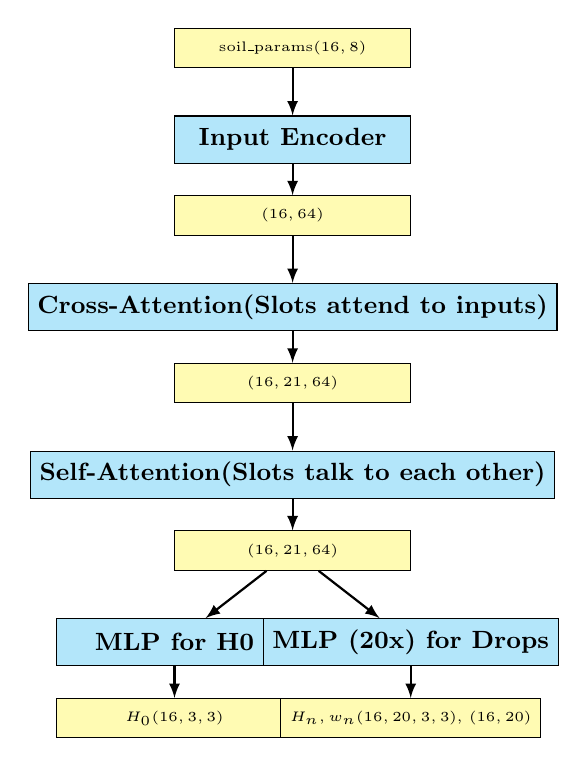
\begin{tikzpicture}[
  proc/.style={rectangle, draw, fill=cyan!30, minimum width=3cm, minimum height=0.6cm, font=\small\bfseries},
  data/.style={rectangle, draw, fill=yellow!30, minimum width=3cm, minimum height=0.5cm, font=\tiny},
  arrow/.style={->, >=latex, thick}
]

\node[data] (in) {soil\_params\\$(16, 8)$};

\node[proc] (enc) [below=0.6cm of in] {Input Encoder};
\draw[arrow] (in) -- (enc);
\node[data] (enc_out) [below=0.4cm of enc] {$(16, 64)$};
\draw[arrow] (enc) -- (enc_out);

\node[proc] (cross) [below=0.6cm of enc_out] {Cross-Attention\\(Slots attend to inputs)};
\draw[arrow] (enc_out) -- (cross);
\node[data] (cross_out) [below=0.4cm of cross] {$(16, 21, 64)$};
\draw[arrow] (cross) -- (cross_out);

\node[proc] (self) [below=0.6cm of cross_out] {Self-Attention\\(Slots talk to each other)};
\draw[arrow] (cross_out) -- (self);
\node[data] (self_out) [below=0.4cm of self] {$(16, 21, 64)$};
\draw[arrow] (self) -- (self_out);

\node[proc] (dec1) [below=0.6cm of self_out, xshift=-1.5cm] {MLP for H0};
\node[proc] (dec2) [below=0.6cm of self_out, xshift=1.5cm] {MLP (20x) for Drops};
\draw[arrow] (self_out) -- (dec1);
\draw[arrow] (self_out) -- (dec2);

\node[data] (h0) [below=0.4cm of dec1] {$H_0$\\$(16,3,3)$};
\node[data] (drops) [below=0.4cm of dec2] {$H_n, w_n$\\$(16,20,3,3)$, $(16,20)$};
\draw[arrow] (dec1) -- (h0);
\draw[arrow] (dec2) -- (drops);

\end{tikzpicture}
\end{figure}

\subsection{Code Logic}

\begin{lstlisting}[caption=Slot-Attention Process]
class SlotAttentionModule(nn.Module):
    def __init__(self, input_dim=8, hidden_dim=64, num_slots=21):
        self.slots = nn.Parameter(torch.randn(num_slots, hidden_dim))
        self.input_encoder = nn.Linear(input_dim, hidden_dim)
        self.cross_attention = MultiheadAttention(hidden_dim, ...)
        self.self_attention = MultiheadAttention(hidden_dim, ...)
        self.mlp_h0 = nn.Sequential(Linear(D), ReLU(), Linear(9))
        self.mlp_drops = nn.Sequential(Linear(D), ReLU(), Linear(10))

    def forward(self, inputs):  # inputs: (16, 8)
        # Encode inputs
        x = ReLU(self.input_encoder(inputs))  # (16, 64)

        # Cross-attention: slots look at input features
        attended = self.cross_attention(
            query=self.slots,  # What do slots want?
            key=x, value=x      # What info exists?
        )  # (16, 21, 64)

        # Self-attention: slots coordinate
        refined = self.self_attention(
            query=attended, key=attended, value=attended
        )  # (16, 21, 64)

        # Decode to stiffness
        H0 = self.mlp_h0(refined[:, 0, :]).reshape(16, 3, 3)

        H_drops, w_gates = [], []
        for n in range(20):
            out = self.mlp_drops(refined[:, n+1, :])
            H_n = out[:, :9].reshape(16, 3, 3)
            w_n = Sigmoid(out[:, 9])
            H_drops.append(H_n)
            w_gates.append(w_n)

        return H0, torch.stack(H_drops, 1), torch.stack(w_gates, 1)
\end{lstlisting}

\subsection{Key Details}

\begin{itemize}
  \item \textbf{21 slots}: 1 for $H_0$ (initial stiffness) + 20 for degradation drops
  \item \textbf{Cross-attention}: Each slot learns which soil parameters matter
    \begin{itemize}
      \item Example: Slot 1 learns ``$H_0$ depends on $G_{\max}$ and $EI$''
      \item Query: slots, Key/Value: soil parameters
    \end{itemize}
  \item \textbf{Self-attention}: Slots don't duplicate work
    \begin{itemize}
      \item Slot 2 specializes in first degradation drop
      \item Slot 3 specializes in second drop, etc.
    \end{itemize}
  \item \textbf{Output}:
    \begin{itemize}
      \item $H_0 \in (16, 3, 3)$: Initial stiffness (3 DOF: lateral, rotation, coupling)
      \item $H_n \in (16, 20, 3, 3)$: 20 stiffness drops
      \item $w_n \in (16, 20)$: Activation weights $\in [0, 1]$ (sigmoid)
    \end{itemize}
\end{itemize}

\section{Component 2: Stiffness Evolution}

\subsection{What It Does}

Apply TIM formula to compute degraded foundation stiffness.

\subsection{Formula}

\begin{equation}
H_{\text{evolved}}[b] = H_0[b] - \sum_{n=1}^{20} w_n[b] \cdot H_n[b]
\end{equation}

Where:
\begin{itemize}
  \item $H_0$: Initial stiffness (tangent)
  \item $H_n$: Plastic drop at yield surface $n$
  \item $w_n \in [0, 1]$: Soft activation gate (smooth triggering)
\end{itemize}

\subsection{Code Logic}

\begin{lstlisting}[caption=Stiffness Evolution]
class StiffnessEvolution(nn.Module):
    def forward(self, H0, H_drops, w_gates):
        # H0: (16, 3, 3)
        # H_drops: (16, 20, 3, 3)
        # w_gates: (16, 20)

        degradation = torch.zeros_like(H0)  # (16, 3, 3)

        for n in range(20):
            # Broadcast: (16, 1, 1) * (16, 3, 3) = (16, 3, 3)
            weight = w_gates[:, n].unsqueeze(-1).unsqueeze(-1)
            degradation += weight * H_drops[:, n]

        H_evolved = H0 - degradation  # TIM formula
        return H_evolved  # (16, 3, 3)
\end{lstlisting}

\subsection{Physical Interpretation}

\begin{figure}[H]
\centering
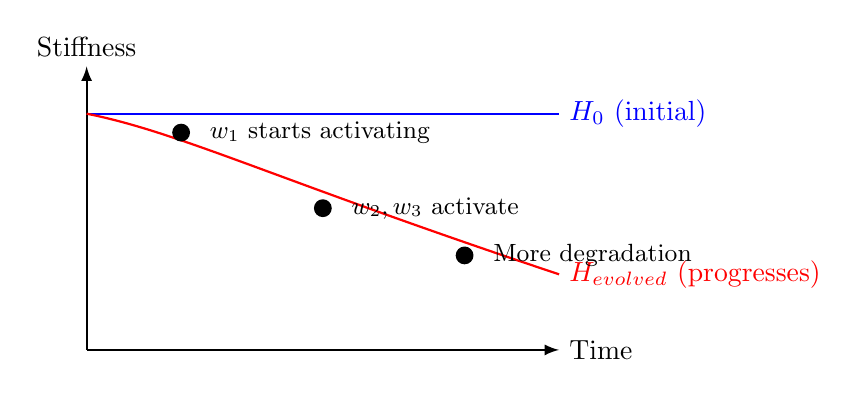
\begin{tikzpicture}[
  scale=1.2,
  axis/.style={->, >=latex, thick},
  curve/.style={thick, blue}
]

% Axes
\draw[axis] (0, 0) -- (5, 0) node[right] {Time};
\draw[axis] (0, 0) -- (0, 3) node[above] {Stiffness};

% Initial stiffness line
\draw[curve] (0, 2.5) -- (5, 2.5) node[right] {$H_0$ (initial)};

% Degradation curve
\draw[curve, red] (0, 2.5) .. controls (1, 2.3) and (2, 1.8) .. (5, 0.8)
  node[right] {$H_{evolved}$ (progresses)};

% Annotations
\node[circle, fill=black, inner sep=0.08cm] at (1, 2.3) {};
\node[right, font=\small] at (1.2, 2.3) {$w_1$ starts activating};

\node[circle, fill=black, inner sep=0.08cm] at (2.5, 1.5) {};
\node[right, font=\small] at (2.7, 1.5) {$w_2, w_3$ activate};

\node[circle, fill=black, inner sep=0.08cm] at (4, 1) {};
\node[right, font=\small] at (4.2, 1) {More degradation};

\end{tikzpicture}
\end{figure}

\textbf{Interpretation:}
\begin{itemize}
  \item Initially all $w_n \approx 0 \Rightarrow H_{\text{evolved}} \approx H_0$ (fresh)
  \item As loads increase: $w_n$ increases smoothly (sigmoid activation)
  \item More gates activate: more degradation
  \item Foundation progressively weakens (realistic failure)
\end{itemize}

\section{Component 3: Load Embedding}

\subsection{What It Does}

Convert 1D load values to 64D embeddings + add temporal position awareness.

\subsection{Schematic}

\begin{figure}[H]
\centering
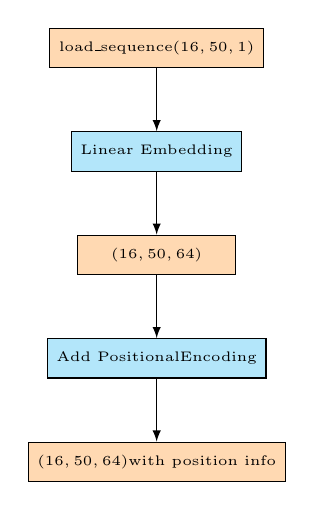
\begin{tikzpicture}[
  node distance=0.8cm,
  box/.style={rectangle, draw, minimum width=2cm, minimum height=0.5cm, font=\tiny},
  emb/.style={box, fill=orange!30},
  encod/.style={box, fill=cyan!30}
]

\node[emb] (in) {load\_sequence\\$(16,50,1)$};

\node[encod, below=of in] (embed) {Linear Embedding};
\draw[->, >=latex] (in) -- (embed);

\node[emb, below=of embed] (emb_out) {$(16,50,64)$};
\draw[->, >=latex] (embed) -- (emb_out);

\node[encod, below=of emb_out] (posenc) {Add Positional\\Encoding};
\draw[->, >=latex] (emb_out) -- (posenc);

\node[emb, below=of posenc] (final) {$(16,50,64)$\\with position info};
\draw[->, >=latex] (posenc) -- (final);

\end{tikzpicture}
\end{figure}

\subsection{Positional Encoding Formula}

\begin{equation}
\text{PE}(t, 2i) = \sin(t / 10000^{2i/D}), \quad \text{PE}(t, 2i+1) = \cos(t / 10000^{2i/D})
\end{equation}

Where:
\begin{itemize}
  \item $t$: time step (0 to 49)
  \item $i$: dimension index (0 to 31)
  \item $D = 64$: embedding dimension
\end{itemize}

\subsection{Code Logic}

\begin{lstlisting}[caption=Load Embedding with Positional Encoding]
# Create embedding layer
embed_layer = nn.Linear(1, 64)

# Create positional encoding (pre-computed)
pos_enc = torch.zeros(50, 64)
for t in range(50):
    for d in range(64):
        if d % 2 == 0:
            pos_enc[t, d] = math.sin(t / (10000 ** (d/64)))
        else:
            pos_enc[t, d] = math.cos(t / (10000 ** (d/64)))

# Apply embedding and add position
embedded = embed_layer(load_sequence)  # (16, 50, 1) -> (16, 50, 64)
embedded = embedded + pos_enc  # Add positional info
# Result: (16, 50, 64) with temporal awareness
\end{lstlisting}

\subsection{Why Positional Encoding?}

\begin{itemize}
  \item Transformers have NO inherent notion of sequence order
  \item Positional encoding tells: ``Position 0 is different from position 5''
  \item Sine/cosine pattern allows learning relative distances
  \item Example: Position 10 and 11 have slightly different encodings
\end{itemize}

\section{Component 4: Concatenation}

\subsection{What It Does}

Merge stiffness information with load time series into unified sequence.

\subsection{Schematic}

\begin{figure}[H]
\centering
\begin{tikzpicture}[
  node distance=0.6cm,
  proc/.style={rectangle, draw, fill=blue!20, minimum width=2.2cm, minimum height=0.5cm, font=\tiny},
  data/.style={rectangle, draw, fill=green!20, minimum width=2.2cm, minimum height=0.45cm, font=\tiny}
]

\node[data] (loads) {Embedded Loads\\$(16,50,64)$};
\node[data, right=0.5cm of loads] (stiff) {Stiffness\\$(16,3,3)$};

\node[proc, below=0.6cm of loads, xshift=0.5cm] (flatten) {Flatten\\9→(16,9)};
\draw[->, >=latex] (stiff) -- (flatten);

\node[proc, below=0.4cm of flatten] (emb) {Embed stiff\\(16,64)};
\draw[->, >=latex] (flatten) -- (emb);

\node[data, below=0.4cm of emb] (token) {Stiff Token\\$(16,1,64)$};
\draw[->, >=latex] (emb) -- (token);

\node[proc, below=0.8cm of loads] (cat) {Concatenate\\along seq dim};
\draw[->, >=latex] (loads) -- (cat);
\draw[->, >=latex] (token) -- (cat);

\node[data, below=0.4cm of cat] (out) {Combined\\$(16,51,64)$\\[token|load1|load2|...|load50]};
\draw[->, >=latex] (cat) -- (out);

\end{tikzpicture}
\end{figure}

\subsection{Code Logic}

\begin{lstlisting}[caption=Concatenation Process]
# Flatten and embed stiffness
H_flat = H_evolved.reshape(16, 9)  # (16, 3, 3) -> (16, 9)
stiff_embed_layer = nn.Linear(9, 64)
H_token = stiff_embed_layer(H_flat)  # (16, 64)
H_token = H_token.unsqueeze(1)  # (16, 1, 64)

# Concatenate along sequence dimension (dim=1)
combined = torch.cat([H_token, embedded_loads], dim=1)
# Position 0: Stiffness context token (16, 1, 64)
# Positions 1-50: Load time series (16, 50, 64)
# Result: (16, 51, 64)
\end{lstlisting}

\subsection{Why Concatenate?}

\begin{itemize}
  \item Transformer needs foundation state context
  \item Different foundations respond differently to same load
  \item Stiffness token at position 0: All loads can attend to it
  \item Transformer learns: ``How do loads affect soft vs stiff foundation?''
\end{itemize}

\section{Component 5: Transformer Encoder}

\subsection{What It Does}

Process all 51 tokens (stiffness + 50 loads) with self-attention.

\subsection{Schematic}

\begin{figure}[H]
\centering
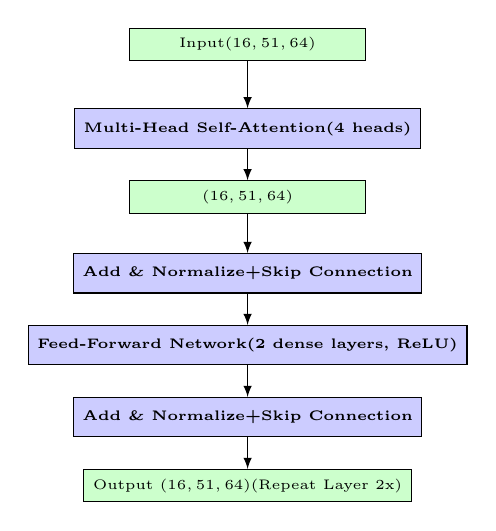
\begin{tikzpicture}[
  scale=0.9,
  layer/.style={rectangle, draw, fill=blue!20, minimum width=3cm, minimum height=0.5cm, font=\tiny\bfseries},
  data/.style={rectangle, draw, fill=green!20, minimum width=3cm, minimum height=0.4cm, font=\tiny}
]

\node[data] (in) {Input\\$(16,51,64)$};

\node[layer, below=0.6cm of in] (sa) {Multi-Head Self-Attention\\(4 heads)};
\draw[->, >=latex] (in) -- (sa);

\node[data, below=0.4cm of sa] (sa_out) {$(16,51,64)$};
\draw[->, >=latex] (sa) -- (sa_out);

\node[layer, below=0.5cm of sa_out] (norm1) {Add \& Normalize\\+Skip Connection};
\draw[->, >=latex] (sa_out) -- (norm1);

\node[layer, below=0.4cm of norm1] (ff) {Feed-Forward Network\\(2 dense layers, ReLU)};
\draw[->, >=latex] (norm1) -- (ff);

\node[layer, below=0.4cm of ff] (norm2) {Add \& Normalize\\+Skip Connection};
\draw[->, >=latex] (ff) -- (norm2);

\node[data, below=0.4cm of norm2] (out) {Output $(16,51,64)$\\(Repeat Layer 2x)};
\draw[->, >=latex] (norm2) -- (out);

\end{tikzpicture}
\end{figure}

\subsection{Attention Mechanism}

\begin{equation}
\text{Attention}(Q, K, V) = \text{softmax}\left(\frac{QK^T}{\sqrt{D}}\right)V
\end{equation}

Where:
\begin{itemize}
  \item $Q$ (Query): ``What do I need?'' (each position looks)
  \item $K$ (Key): ``What info is available?'' (what exists?)
  \item $V$ (Value): ``What are actual values?'' (weighted sum)
  \item $\sqrt{D} = 8$ (scaling for numerical stability)
\end{itemize}

\subsection{Key Properties}

\begin{itemize}
  \item \textbf{Self-attention}: Each position attends to ALL 51 positions
  \item \textbf{Global context}: Stiffness at position 0 can influence position 50
  \item \textbf{4 heads}: Learn 4 different attention patterns simultaneously
  \item \textbf{2 layers}: Stack 2 encoder layers for deeper processing
  \item \textbf{Skip connections}: Preserve original information while processing
\end{itemize}

\subsection{What It Learns}

\begin{itemize}
  \item Which loads are important (high attention weights)
  \item How loads interact with foundation stiffness
  \item Long-range dependencies (load at $t=5$ affects $t=45$)
  \item Complex nonlinear relationships
\end{itemize}

\section{Component 6: Transformer Decoder}

\subsection{What It Does}

Generate output using cross-attention to encoder information.

\subsection{Schematic}

\begin{figure}[H]
\centering
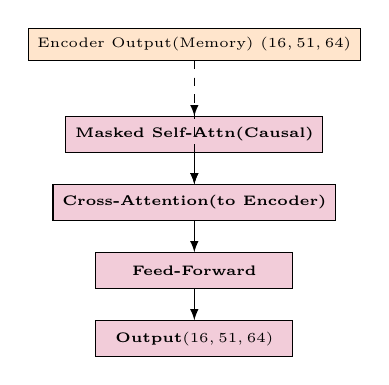
\begin{tikzpicture}[
  scale=0.9,
  layer/.style={rectangle, draw, fill=purple!20, minimum width=2.5cm, minimum height=0.45cm, font=\tiny\bfseries},
  memory/.style={rectangle, draw, fill=orange!20, minimum width=2.5cm, minimum height=0.4cm, font=\tiny}
]

\node[memory] (enc_mem) {Encoder Output\\(Memory) $(16,51,64)$};

\node[layer, below=0.7cm of enc_mem] (msa) {Masked Self-Attn\\(Causal)};
\draw[->, >=latex, dashed] (enc_mem) -- (msa);

\node[layer, below=0.4cm of msa] (ca) {Cross-Attention\\(to Encoder)};
\draw[->, >=latex] (msa) -- (ca);
\draw[->, >=latex, dashed] (enc_mem) -- (ca);

\node[layer, below=0.4cm of ca] (ff) {Feed-Forward};
\draw[->, >=latex] (ca) -- (ff);

\node[layer, below=0.4cm of ff] (out) {Output\\$(16,51,64)$};
\draw[->, >=latex] (ff) -- (out);

\end{tikzpicture}
\end{figure}

\subsection{Masked Self-Attention}

\textbf{Why masked?} Prevent looking at future information.

\begin{equation}
\text{scores}_{ij} = \begin{cases}
\frac{QK^T}{\sqrt{D}} & \text{if } j \leq i \\
-\infty & \text{if } j > i
\end{cases}
\end{equation}

After softmax: position $i$ only attends to positions $\leq i$.

\subsection{Cross-Attention}

Query comes from decoder, Key/Value from encoder:
\begin{itemize}
  \item Decoder asks: ``What did encoder learn about this info?''
  \item Encoder provides: All 51 processed positions
  \item Result: Decoder combines past predictions with encoder context
\end{itemize}

\section{Component 7: Frequency Head}

\subsection{What It Does}

Convert decoder output to single frequency prediction.

\subsection{Schematic}

\begin{figure}[H]
\centering
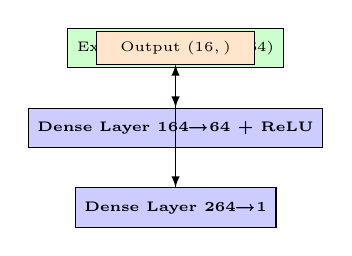
\begin{tikzpicture}[
  node distance=0.5cm,
  proc/.style={rectangle, draw, fill=blue!20, minimum width=2cm, minimum height=0.5cm, font=\tiny\bfseries}
]

\node[rectangle, draw, fill=green!20, minimum width=2cm, minimum height=0.5cm, font=\tiny] (in) {Extract Token 0\\$(16,64)$};

\node[proc, below=of in] (dense1) {Dense Layer 1\\64→64 + ReLU};
\draw[->, >=latex] (in) -- (dense1);

\node[proc, below=of dense1] (dense2) {Dense Layer 2\\64→1};
\draw[->, >=latex] (dense1) -- (dense2);

\node[rectangle, draw, fill=orange!20, minimum width=2cm, minimum height=0.4cm, font=\tiny] (out) {Output $(16,)$};
\draw[->, >=latex] (dense2) -- (out);

\end{tikzpicture}
\end{figure}

\subsection{Code Logic}

\begin{lstlisting}[caption=Frequency Prediction Head]
# Extract first token (stiffness token + context)
freq_token = decoder_output[:, 0, :]  # (16, 64)

# MLP: 64D -> 64D -> 1D
freq_head = nn.Sequential(
    nn.Linear(64, 64),
    nn.ReLU(),
    nn.Linear(64, 1)
)

freq_pred = freq_head(freq_token).squeeze(-1)  # (16,)
\end{lstlisting}

\subsection{Why Token 0?}

\begin{itemize}
  \item Position 0 is the stiffness token (foundation state)
  \item After all attention layers: it's aggregated all load info
  \item Best representative for frequency (which depends on stiffness)
  \item Physical logic: $f_0 = \sqrt{K/M}$ (frequency depends on stiffness)
\end{itemize}

\newpage
\section{Loss Functions}

\subsection{The Goal: Balance Data + Physics}

\begin{table}[H]
\centering
\begin{tabular}{|l|l|c|}
\hline
\textbf{Loss Term} & \textbf{Purpose} & \textbf{Weight} \\
\hline
Data Loss & Fit predictions to measurements & $\alpha = 1.0$ \\
\hline
Frequency Loss & Enforce energy conservation (LoT1) & $\beta = 0.5$ \\
\hline
Monotonicity Loss & Enforce progressive failure (LoT2) & $\gamma = 0.3$ \\
\hline
Positive Stiffness Loss & Prevent invalid matrices (LoT2) & $\delta = 0.2$ \\
\hline
\end{tabular}
\end{table}

\subsection{Loss 1: Data Accuracy}

\begin{equation}
\mathcal{L}_{\text{data}} = \frac{1}{B}\sum_{b=1}^{B} (f_{\text{pred}}^b - f_{\text{true}}^b)^2
\end{equation}

\textbf{Meaning:} How close are predictions to real measurements?

\subsection{Loss 2: Frequency Consistency (Physics)}

\begin{equation}
\mathcal{L}_{\text{freq}} = \frac{1}{B}\sum_{b=1}^{B} (f_{\text{pred}}^b - f_{\text{analytical}}^b)^2
\end{equation}

\textbf{Meaning:} Predicted frequency should match physics-derived frequency.

\subsection{Loss 3: Monotonicity}

\begin{equation}
\mathcal{L}_{\text{mono}} = \frac{1}{B}\sum_{b=1}^{B} \sum_{n=1}^{19} \max(0, w_n^b - w_{n+1}^b)
\end{equation}

\textbf{Meaning:} Activation gates must be ordered: $w_1 \leq w_2 \leq \cdots \leq w_{20}$

\textbf{Physical interpretation:} Foundation fails progressively, not in reverse.

\subsection{Loss 4: Non-Negative Stiffness}

\begin{equation}
\mathcal{L}_{\text{pos}} = \frac{1}{B}\sum_{b=1}^{B} \sum_{i=1}^{3} \max(0, -\lambda_i(H_{\text{evolved}}^b))
\end{equation}

\textbf{Meaning:} All eigenvalues of stiffness matrix must be $\geq 0$ (positive definite).

\textbf{Physical interpretation:} Stiffness matrix must be valid (no ''whiplash'' effects).

\subsection{Composite Loss}

\begin{equation}
\mathcal{L}_{\text{total}} = \alpha \mathcal{L}_{\text{data}} + \beta \mathcal{L}_{\text{freq}} + \gamma \mathcal{L}_{\text{mono}} + \delta \mathcal{L}_{\text{pos}}
\end{equation}

\section{Training Cycle}

\subsection{One Complete Epoch}

\begin{figure}[H]
\centering
\fbox{\begin{minipage}{0.95\textwidth}
\textbf{Epoch $e$: Data $\to$ Update}

\small
\begin{enumerate}
  \item \textbf{Load batch}: 16 scenarios
  \begin{itemize}
    \item load\_sequence $(16, 50, 1)$ - Load histories
    \item soil\_params $(16, 8)$ - Soil properties
    \item true\_freq $(16,)$ - Ground truth
    \item analytical\_freq $(16,)$ - Physics-based target
  \end{itemize}

  \item \textbf{Forward pass}: Data flows through network
  \begin{itemize}
    \item Slot-Attention: soil $\to$ stiffness
    \item Stiffness Evolution: degrade
    \item Embedding: loads $\to (16, 50, 64)$
    \item Concatenation: $(16, 51, 64)$
    \item Encoder: Self-attention
    \item Decoder: Cross-attention
    \item Head: $(16,)$ predictions
  \end{itemize}
  \textbf{Output}: freq\_pred, H\_evolved, w\_gates

  \item \textbf{Loss computation}
  \begin{itemize}
    \item $\mathcal{L}_{\text{data}} = \text{MSE}(\text{pred}, \text{true})$
    \item $\mathcal{L}_{\text{freq}} = \text{MSE}(\text{pred}, \text{analytical})$
    \item $\mathcal{L}_{\text{mono}} = \text{monotonicity\_penalty}(w_{\text{gates}})$
    \item $\mathcal{L}_{\text{pos}} = \text{positive\_stiffness}(H_{\text{evolved}})$
    \item $\mathcal{L}_{\text{total}} = 1.0 \cdot L_d + 0.5 \cdot L_f + 0.3 \cdot L_m + 0.2 \cdot L_p$
  \end{itemize}

  \item \textbf{Backward pass}: Compute gradients
  \begin{itemize}
    \item $\nabla_\theta \mathcal{L}$ for ALL parameters via chain rule
    \item Shapes: Gradients have same shape as parameters
  \end{itemize}

  \item \textbf{Update}: Adam optimizer adjusts parameters
  \begin{itemize}
    \item $\theta_{\text{new}} = \theta_{\text{old}} - 0.001 \times \nabla_\theta \mathcal{L}$
    \item Learning rate = 0.001 (moderately aggressive)
  \end{itemize}

  \item \textbf{Track}: Save metrics for later visualization
  \begin{itemize}
    \item Losses, predictions, stiffness norms
  \end{itemize}
\end{enumerate}
\end{minipage}}
\end{figure}

\subsection{Code: One Epoch}

\begin{lstlisting}[caption=Single Training Epoch]
for epoch in range(10):
    # 1. Load data
    load_seq, soil_p, true_f, anal_f = next(data_loader)

    # 2. FORWARD PASS
    pred_freq, H_evolved = model(load_seq, soil_p)
    H0, H_drops, w_gates = model.calibration(soil_p)

    # 3. LOSS COMPUTATION
    loss_total, loss_dict = loss_fn(
        pred_freq, anal_f, w_gates, H_evolved, true_f,
        alpha=1.0, beta=0.5, gamma=0.3, delta=0.2
    )

    # 4. BACKWARD PASS
    optimizer.zero_grad()      # Clear old gradients
    loss_total.backward()      # Compute new gradients

    # 5. UPDATE
    optimizer.step()           # Update all parameters

    # 6. TRACK
    history['loss'].append(loss_total.item())
    if (epoch+1) % 2 == 0:
        print(f"Epoch {epoch+1}: Loss={loss_total.item():.4f}")

# 7. VISUALIZE
create_visualizations(history)
\end{lstlisting}

\section{Key Insights}

\subsection{Why This Architecture Works}

\begin{table}[H]
\centering
\begin{tabular}{|l|l|}
\hline
\textbf{Challenge} & \textbf{Solution} \\
\hline
Different soil combinations & Slot-Attention learns auto-calibration \\
\hline
Limited experimental data (~30) & Physics losses + FEM pre-training \\
\hline
Complex load sequences & Transformer captures long-range dependencies \\
\hline
Need for interpretability & Attention weights reveal decisions \\
\hline
Physical validity & Physics losses enforce constraints \\
\hline
\end{tabular}
\end{table}

\subsection{Parameter Count}

\begin{itemize}
  \item Slot-Attention: $\sim$30K parameters
  \item Encoder/Decoder: $\sim$200K parameters
  \item **Total**: $\sim$235K parameters (vs BERT: 110M)
  \item Small models: Better with limited data, faster inference
\end{itemize}

\end{document}
